% Options for packages loaded elsewhere
\PassOptionsToPackage{unicode}{hyperref}
\PassOptionsToPackage{hyphens}{url}
%
\documentclass[
  12pt,
  a5,margin=2cmpaper,
]{article}
\usepackage{amsmath,amssymb}
\usepackage{iftex}
\ifPDFTeX
  \usepackage[T1]{fontenc}
  \usepackage[utf8]{inputenc}
  \usepackage{textcomp} % provide euro and other symbols
\else % if luatex or xetex
  \usepackage{unicode-math} % this also loads fontspec
  \defaultfontfeatures{Scale=MatchLowercase}
  \defaultfontfeatures[\rmfamily]{Ligatures=TeX,Scale=1}
\fi
\usepackage{lmodern}
\ifPDFTeX\else
  % xetex/luatex font selection
\fi
% Use upquote if available, for straight quotes in verbatim environments
\IfFileExists{upquote.sty}{\usepackage{upquote}}{}
\IfFileExists{microtype.sty}{% use microtype if available
  \usepackage[]{microtype}
  \UseMicrotypeSet[protrusion]{basicmath} % disable protrusion for tt fonts
}{}
\makeatletter
\@ifundefined{KOMAClassName}{% if non-KOMA class
  \IfFileExists{parskip.sty}{%
    \usepackage{parskip}
  }{% else
    \setlength{\parindent}{0pt}
    \setlength{\parskip}{6pt plus 2pt minus 1pt}}
}{% if KOMA class
  \KOMAoptions{parskip=half}}
\makeatother
\usepackage{xcolor}
\usepackage{graphicx}
\makeatletter
\def\maxwidth{\ifdim\Gin@nat@width>\linewidth\linewidth\else\Gin@nat@width\fi}
\def\maxheight{\ifdim\Gin@nat@height>\textheight\textheight\else\Gin@nat@height\fi}
\makeatother
% Scale images if necessary, so that they will not overflow the page
% margins by default, and it is still possible to overwrite the defaults
% using explicit options in \includegraphics[width, height, ...]{}
\setkeys{Gin}{width=\maxwidth,height=\maxheight,keepaspectratio}
% Set default figure placement to htbp
\makeatletter
\def\fps@figure{htbp}
\makeatother
\setlength{\emergencystretch}{3em} % prevent overfull lines
\providecommand{\tightlist}{%
  \setlength{\itemsep}{0pt}\setlength{\parskip}{0pt}}
\setcounter{secnumdepth}{-\maxdimen} % remove section numbering
\ifLuaTeX
  \usepackage{selnolig}  % disable illegal ligatures
\fi
\IfFileExists{bookmark.sty}{\usepackage{bookmark}}{\usepackage{hyperref}}
\IfFileExists{xurl.sty}{\usepackage{xurl}}{} % add URL line breaks if available
\urlstyle{same}
\hypersetup{
  pdftitle={Gigapixel streaming towards prognosis endpoint},
  pdfauthor={Hans Pinckaersa*, Shephan Doopera, Geert Litjensa},
  hidelinks,
  pdfcreator={LaTeX via pandoc}}

\title{Gigapixel streaming towards prognosis endpoint}
\author{Hans Pinckaers\textsuperscript{a}*, Shephan
Dooper\textsuperscript{a}, Geert Litjens\textsuperscript{a}}
\date{}

\begin{document}
\maketitle

Corresponding author: Hans Pinckaers, Radboud University Medical Center,
Postbus 9101, 6500 HB Nijmegen, The Netherlands (tel +31 634 856 950,
hans.pinckaers@radboudumc.nl)

\textsuperscript{a} Department of Pathology, Radboud Institute for
Health Sciences, Radboud University Medical Center, Nijmegen, The
Netherlands

\hypertarget{introduction}{%
\section{Introduction}\label{introduction}}

In this thesis we want to investigate if histopathology slides contain
additional information to prognosticate patient. In Chapter 2, we showed
that it's possible to optimize towards biochemical recurrence of
prostate cancer. However, this work was done on smaller subregions of
the available slides. This requires sampling high-grade tumor regions,
and only performing the algorithm in those. Besides, it's likely that
there is information outside this region that could contain signal for
prognostication of the patient, e.g., perineural growth.

Given the streaming method of Chapter 3, and the prostate cancer
classification performance shown in Chapter 4, a natural next step would
be to optimize a CNN on whole-slide images on a cohort of prostate
cancer patients to a survival endpoint. We started on this endeavor and
we would like to present preliminary results here.

\hypertarget{the-data}{%
\section{The data}\label{the-data}}

At our hospital, we collected a cohort of patient of 903 patients which
underwent prostatectomy, with follow-up information. Primary endpoint
for this cohort was biochemical recurrence. This dataset, collected by
the Urology department recorded biochemical recurrence by monitoring
ordered lab tests of included patients. Patients treated in the
hospital, between 1992 and 2012 were included. These tests were ordered
by treating physicians in the hospital, or outside by general
practitioners. Generally, after one year of follow-up, patients were
transferred to their general practitioner for monitoring.

Tissue slides were picked from the hospital archive containing the
highest grade tumor, based on the pathology reports. Slides were scanned
into whole-slide images on a 3DHistech P1000 scanner, at 0.25mu/px
resolution. The number of slides ranged from 1 to 9 per patient, with a
median of two slides. Before streaming the slides, the tissue on the
slides was combined to create one image with all the tissue. This could
result in multiple gigapixel-sized images.

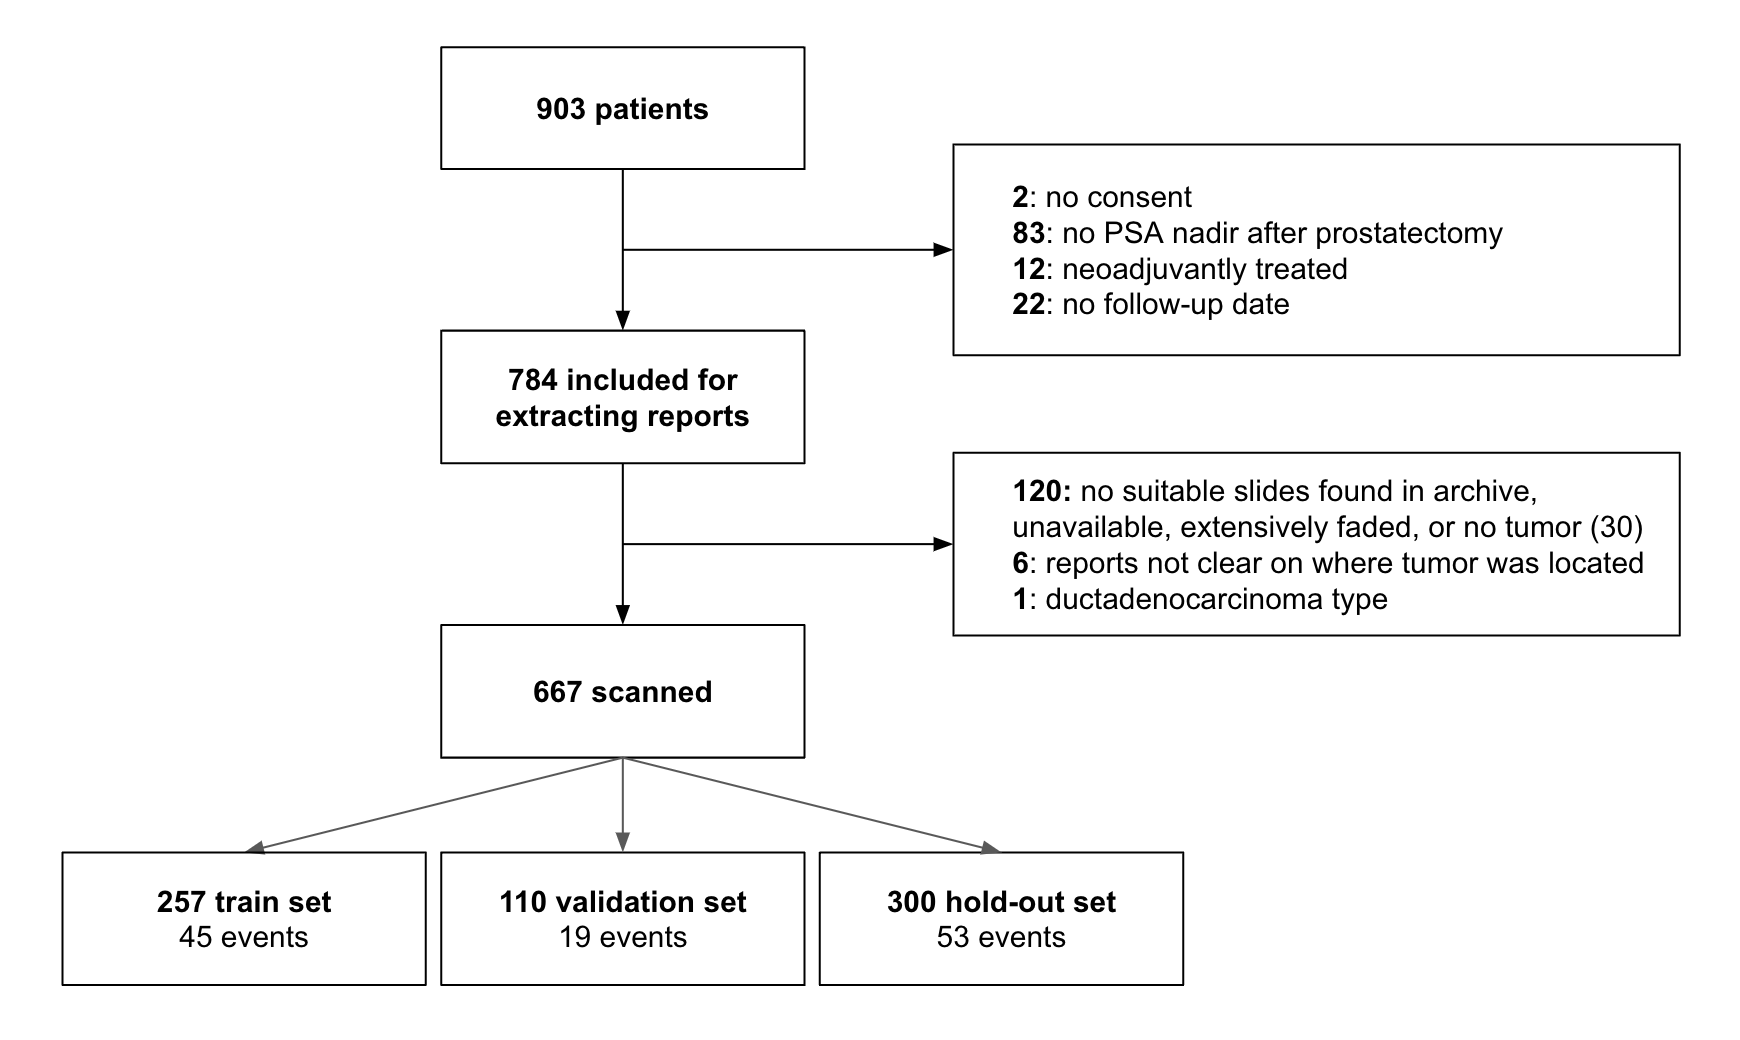
\includegraphics{chpt5_imgs/inclusion.png}

\hypertarget{experimental-setup}{%
\section{Experimental setup}\label{experimental-setup}}

We divided this cohort into three sets; a train set, consisting of 257
patients (with 45 biochemical recurrence events), a limited validation
set (110 patients, 19 events) and a hold-out set (296 patients, 52
events). Due to scanner or corrupt whole-slide image files, we had to
exclude an additional four patients.

We leveraged the streaming implementation of chapter 2 to optimize a
imagenet-pretrained ResNet34 with a attention-based regression head,
following Dooper, \emph{et al.}{[}cite Stephan Dooper, CLAM{]}. Between
the regression had and the ResNet34, we reduced the dimensionality of
the feature map with a 4x4 maxpool layer.

We divided the training into two phases. In the first phase, we only
optimized the attention head with the ResNet frozen. During training, we
cropped the images to one gigapixel (32768), to speed up and regularize
the training. We used SGD-momemtum with a learning rate of 3e-6,
streaming tile size 7680, the minitbatch-size was 20. The first phase
converged after 300 epochs. We optimized towards time-to-event following
chapter 4, using the Huber loss.

The second phase started by unfreezing ResNet34. We slightly dropped the
learning rate to 1e-6. The network began overfitting around 10 epochs,
we picked the checkpoint at epoch 8 for evaluation, based on validation
set performance. We used weight averaging over the last five epochs as
explained in chapter 3.

Given time constraints, we couldn't perform further hyperparameter
tuning or experimentation.

\hypertarget{results}{%
\section{Results}\label{results}}

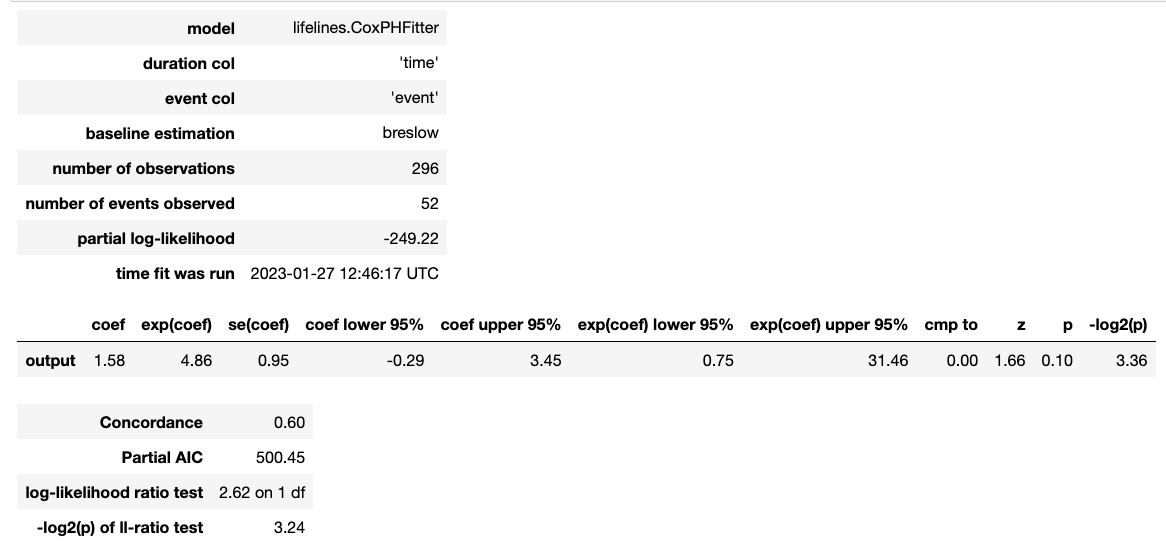
\includegraphics{chpt5_imgs/results.png}
\includegraphics{chpt5_imgs/results_notnormalized.png}

Univariate Cox proportional hazard analysis, gives a hazard ratio of
1.83 with a p-value of 0.10, with an output range of 0 to 2.6.
Normalizing the range gives a hazard ratio of 4.86. The concordance is
0.6.

TODO: multivariate TODO: image only / clin only / fusion

Figure 2 shows the concordance of a CoxPH statistical analysis using the
neural network output.

\includegraphics{chpt5_imgs/concordance.png}

\includegraphics{chpt5_imgs/heatmap.jpeg}
\includegraphics{chpt5_imgs/heatmapwithout.jpeg}

\hypertarget{discussion}{%
\subsubsection{Discussion}\label{discussion}}

This work in progress explored the hypothesis that whole-slide images
can be used to predict prognosis. We analyzed whole-slide images of a
population cohort of patients who had undergone prostatectomy. We
attempted to predict the time to biochemical recurrence for these
patients. Although we could not achieve statistically significant
results due to the size of the dataset, there was a discernible signal
in the slides. Using explainability methods, we demonstrated that the
network focuses on the tumor.

Future work could focus on using survival based losses.

As shown in Figure 2, in agreement with chapter 2, training with a small
dataset of very high-resolution images was remarkably stable.

This preliminary assessment lays the groundwork for fully learning
end-to-end, clinically interesting endpoints from histology images while
harnessing the full potential of neural networks to find relevant
features without manual feature engineering. One could argue that
working on patches adds assumptions to the task and lacks context due to
cropping the slide. However, deep learning has shown that neural
networks can learn these assumptions and signals themselves, given
enough data and appropriate labels.

\textbf{Acknowledgments}

\emph{Wouter Bulten}

\textbf{References}

\end{document}
